\chapter{Theory}
\setcounter{page}{1}
\pagenumbering{arabic}
\section{Numerical Weather Prediction Model}
\p
Modern weather prediction always bases on use of output from Numerical Weather Prediction~(\emph{NWP}) models. To improve the quality of these predictions, one has to assess possible errors in the NWP-models. First the procedure of a NWP-model will be described.\cite{grandy2004time}
\p
To initialize the numerical model, information about the current state of the atmosphere (and other modelled systems) is needed. These initial values have to be given in the \glqq model space\grqq. Meaning, that all values describing the system are needed in the way the model would produce them on every grid point.
\p
Due to practical reasons, there can't take place measurements of the state of the atmosphere on every grid point in the 3D-Atmosphere multiple times a day for every weather forecast. To introduce a possibility to start a NWP-model nevertheless, the process of data assimilation is used.
\section{Data Assimilation}
\p
Main objective of the data assimilation process is to find a model state, for that holds, that the forecast of the NWP-model will be closest possible to the physical truth. This objective differs from the task, to find a model state closest to the current/initial, true atmospheric state.
\p
Another problem addressed by the data assimilation process is the presence of measurement errors. Already small errors in a single measurement can imply extensive imbalances and thereby erroneous processes in the forecast. Therefore it is important to damp the influence of any single measurement in favor of correct balancing and hence a correct representation of physical processes in the model.
\p 
To realize both objectives of data assimilation, a model run is started about one hour before the forecast is to be produced. As initial condition a forecast for that point in time is used. In the timeframe between start of the model run and start of the forecast process, the data assimilation takes place. During this process all available measurements are being incorporated in the model. The way this is done depends on the specific data assimilation scheme choosen. 
\subsection{Observation Nudging (COSMO)}
\p
One particular assimilation scheme is the \emph{observation-nudging}. This scheme is used in the COSMO-model. In this scheme the incorporation is realized by a change of the prognostic tendency produced by the model during forward integration. The change for any observed variable $\phi(x,t)$ by $k$th observation is given by(\cite{cosmo_da}):
\begin{equation}
\frac{\partial}{\partial\!t}\phi(\vb{x},t) = F(\phi,\vb{x},t)+ G_\phi \ftimes \sum_{k_{(obs)}}W_k(\vb{x},t)\ftimes \qty[\phi_k^{obs}-\phi(x_k,t)] \label{eq:cosmo_nudging1}
\end{equation}
\p
Where $F$ is the tendency produced by model dynamics and physics, $G$ a variable dependent constant, $W_k$ a observation depend weight decreasing with distance from the observation in space and time and $\phi^{obs}$ the observed value. By this procedure the model is forced to stay close to observated values where these are available but can develop free where no information is known.
\p
If the model physics and dynamics \(F(\cdots)\) were zero, the assimilation terms would produce a exponential convergence of \(\phi\) to \(\phi^{obs}\). To guarantee, that the modeled system is still conform to the physical model, the assimilation term should be small compared to the model physics and dynamics. To ensure this, $W_k$ is being adjusted with the formula:
\begin{equation} 
W_k=\frac{w_k+1}{\sum_j w_j+1}\ftimes w_k \label{eq:cosmo_nudging2}
 \end{equation}
\p
Where the individual measurements weight $w_k$ is being limited by the utilization of the sum over all influencing weights $w_j$
\p
An advantage of this method is, that measurements can flexibly be added to the assimilation process whenever they are available while other methods are only able to incorporate additional information at fixed times.
\p
For nudging based assimilation the measured \glqq truth\grqq\ has to been known in model space (see \(\phi\) in \eqref{eq:cosmo_nudging1}), thus no satellite data can effectively be used in data assimilation.
\p
Also the incorporation of radar precipitation data needs special procedure called \emph{latent heat nudging}. It would not be effective to just add the precipitation observed where the model is not producing it, as the precipitation would just fall to the ground without adjusting the model dynamics effectively. This would just be fixing the symptoms but not the cause of a lack of precipitation.
\p
To fix the cause of a lack or excess of precipitation latent heat is added or removed from the lower bound of clouds. This will then increase or reduce vertical motion in the cloud and then cause an adjustment of the precipitation rate in the needed direction.
\p
While the observation nudging scheme is rather pragmatically designed it shows best performance in operational weather forecasts due to its high adjustability. Also the forecasting framework is easier to set up. Operationally the model is always in \glqq data assimilation\grqq mode, and as soon as no observations are available anymore the model will automatically be running as free model -- the second righthand term in \eqref{eq:cosmo_nudging1} will be zero.
\p
Also this scheme allows the model during data assimilation to move to its attractor, and therefore minimizing spin up errors (see section \ref{sec:SpinUp}). 
\subsection{Ensemble Kalman Filter (WRF)}
\p
Another approach of data assimilation is chosen in the WRF data assimilation program called \emph{DART}. The Ensemble Kalman Filter is based on the original by Kalman introduced Kalman Filter.
\p 
The Kalman Filter works on linear systems. The initial conditions are not exactly known but their probability distribution is. Also measurements after a certain time and their error distribution are known. The Kalman Filter then proceeds in two steps.
\begin{itemize}
\item First from the initial condition a forecast is produced. Because of the linearity the propagation of the uncertainty is feasible computable. The result is called the bayesian prior.
\item Second the measurements and their uncertainty, called bayesian posterior, are taken into account.  Utilizing Bayes' Theorem both the prior and the posterior are combined to the assimilation.
\end{itemize}
\p
From this assimilation output now again a forecast can be started, which then in combination with new measurements allows to \emph{cycle} the assimilation scheme. For systems with normal distributed errors, this scheme is known to produce the optimal solution.
\p
In numerical weather prediction however the dynamic system is very strongly not linear. This makes it infeasible to predict the propagation of uncertainty with time as the Fokker-Planck equations would have to be solved. The usage of the Ensemble Kalman Filter avoids this tedious task at the cost of losing the property of optimal solution.
\p
The Ensemble Kalman Filter utilizes a bootstrapping method to simulate a solution of the Fokker-Planck equations. To achieve this, the initial uncertainty is represented by a sample $\order{\textit{\numrange{50}{100}}}$ of initial conditions whose variance is maximized along the Lyapunov vectors with biggest Lyapunov exponents.
\section{Model Error}
While there is obvious description of what a model error is, namely a discrepancy between the forecast and the actual physical development, there are different concepts of describing model errors.
\p
From a perspective of model development there are three kinds of errors. First of all there are approximations and neglections consciously implemented into the numerical model. These errors are taken into account to allow computability in a certain timeframe as the forecast always has to be computed faster than the forecasted event takes place. A second source of error are uncertainties in parameters, boundary and initial data, and measurement errors. These errors are thought to be countered by data assimilation and ensemble forecasting. The third source of errors are implementation errors. This is expressed by differences between the formal \glqq numerical model\grqq\ and the model actually implemented by the source code.
\p                                
One insightful way of describing model errors follows \cite{judd2008geometry}. Judd describes different types of errors by their origin, neglecting whether they're distinguishable later. He also describes the data assimilation process not as independent, but as part of the model.
\subsection{Initialisation Error}
\p
One widely known source of error is error in the initial data. Often it is assumed, that uncertainty of the initial state will grow even in a perfect model exponentially with time. \cite{smith1999uncertainty} however finds, that this behavior will not always be observed. 
\p In dissipative systems \emph{sometimes} a initialization error will be dissipated and the model trajectory will converge to the real one. However \emph{statistically} the assumption of an exponential error growth due to initialization errors still holds.
\p
Another implication of the exponential growth is, that for a certain time after the beginning the errors due to initialization errors will be small compared to other errors.
\subsection{Spin Up Error}
\label{sec:SpinUp}
\p
Both numerical models as the physical climate are describable by a multidimensional attractor \citep{judd2008geometry}. For the physical climate this attractor implies a recurrence time of $\order{\SI{e30}{\years}}$ for which the climate system would return to a similar state. The spatial dimension of this attractor is with $\order{\textit{\numrange{e5}{e6}}}$ also too big to be imagined or visualized.
\p
It is observed, that numerical weather models will be strongly attracted to an attractor, which might differ from the physical climate attractor. If a difference between the physical and the model attractor exist and the model is initialized in a state lying on the physical attractor, in the beginning of the simulation the model will move from the physical attractor to the intrinsic attractor of the numerical model, resulting in erroneous tendencies called \emph{spin up}.
\p
Spin up errors can also occur due to artificial different treatment of the first time steps of numerical modeling. This can be implemented as simplification or by error.
\p
Spin up errors can be reduced by using appropriate data assimilation. To minimize the time model output is influenced by spin up it's important to use the same model system in data assimilation as will be used for simulation. Also model configuration (choice of parametrizations) has to be equal. Otherwise the spin up process can need more then several days, dominating the whole forecasting time. 
\subsection{Tendency Error}
\p
A numerical forecast model might also exhibit constant error in tendencies of variables. This kind of error differs from spin up as tendency errors don't diminish with longer forecast periods letting the actual error grow larger and larger.
\p
As this kind of error often implies a breaking of conservation laws of energy or similar these errors are either included by mistake or by neglection of processes in the atmosphere. Examples for such processes might be aerosols, 3D-radiation scattering or sound waves.
\p
Weather forecast models with higher resolution often don't run for more than a few days therefore small tendency errors might not grow large or are indistinguishable from spin up effects.
\section{Reforecasts}
\p
One complication in the evaluation process of numerical weather model used in production is inconsistency over time. For the production use of weather services mistakes in the model are fixed as soon as possible. However this leads incomparability of model behavior over longer time scales.
\p
To develop a deeper understanding of model behavior \emph{reforecasts} are used. Therefor the model is started from initialization states in the past and a forecast for the past is produced. This method differs from a reanalysis as here during the forecast no measurements are incorporated into the model.
\p
By freezing on a specific model configuration and re-evaluation of free forecasts from reanalysis initial data, one can investigate the attractor of the numerical model.
\p
There are different applications imaginable for utilizing reforecasts for model evaluation. [?] compared the model output to measurements and [?] investigated physical properties of the climate exhibited by the model in terms of humidity fluxes [?] as in terms of conservation properties [?].
\p
The initial data used from the HeRZ-reanalyses are in this work considered as free from systematic biases. With this assumption no errors can be found, that are not constrainable by measurements during data assimilation. 
\pagebreak
\section{Initial Tendency Method}
\p
Objective of the evaluation method used in this work is to evaluate the models without the use of additional measurements. This kind of evaluation has to verify intrinsic physical properties or the general behavior of the model.
\p
Under the assumption of a stationary climate one can assume, that statistically all variables have to be constant. This is expectably true for extensive or intensive variables.
\p
The time scales for which different variables in the climate system are quasi constant can become very large. Also variables that vary with the diurnal cycle would cause problems, if the diurnal cycle isn't resolved by the model starting times. If the model is for example only started at the local morning, the tendencies for temperature would always be positive whereas this doesn't point to erroneous behavior of the model. It is important to note that the diurnal cycle might not be resolved by a 6-horal sampling.
\p
Due to this for this evaluation known tendencies of all variables will be subtracted before averaging. To determine the known tendencies the reanalysis from which the model is started are used to calculate the real background tendencies.
\p

For a Variable $\Phi$ let $\Phi^R_0$ be the reanalysis field from which the model is started and $\Phi^R_1$ the next reanalysis field available after a time of $\Delta T$.
\p
 The forecast field for $t$ seconds after $\Phi^R_0$ is denoted $\Phi^M(t)$. The model time step numbered $0\leq i\leq n \in \mathbb{N}$ is $\Delta t$ seconds. Therefore model fields are available for $t=i\Delta t$ and called $\Phi^M_i$.
 \p
The Background tendency is $\dot{\Phi}^R=\nicefrac{(\Phi^R_1-\Phi^R_0)}{\Delta T}$ if $i<\nicefrac{\Delta T}{\Delta t}$, elsewise $\Phi^R_{2,3,\cdots}$ will be used such that the time step $i$ is in between the used reanalyses.
 The model tendency $\dot{\Phi}_i$ exclusive the background tendency between the time steps $i$ and $i+1$ is then calculated by:
\begin{equation}
\dot{\Phi}_i=\frac{\Phi^M_{i+1}-\Phi^M_i}{\Delta t}-\dot{\Phi}^R
\end{equation}
\p
Occasionally due to practical reasons some model tendencies $\dot{\Phi}_i$ to $\dot{\Phi}_j$ will be examined only averaged:
\begin{equation}
\dot{\Phi}_{ij}=\frac{1}{j-i}\sum_{k=i}^{j-1}\dot{\Phi}_k=\frac{\Phi^M_{j}-\Phi^M_i}{(j-i)\Delta t}-\dot{\Phi}^R\qqtext{with:} i<j\leq n
\end{equation}
\p
For some variables the model can be configured or adapted to add different tendency terms, that are normally are integrated, directly to the model output. This then allows for another way to compute $\dot{\Phi}_i$:
\begin{equation}
\dot{\Phi}_i+\dot{\Phi}^R=\sum_k \dot{\varphi}^M_k
\end{equation}
\p
Here $\dot{\varphi}^M_k$ are the different model tendencies from the dynamics and physics of the NWP. It is important that all processes are included for this equation to hold.\\
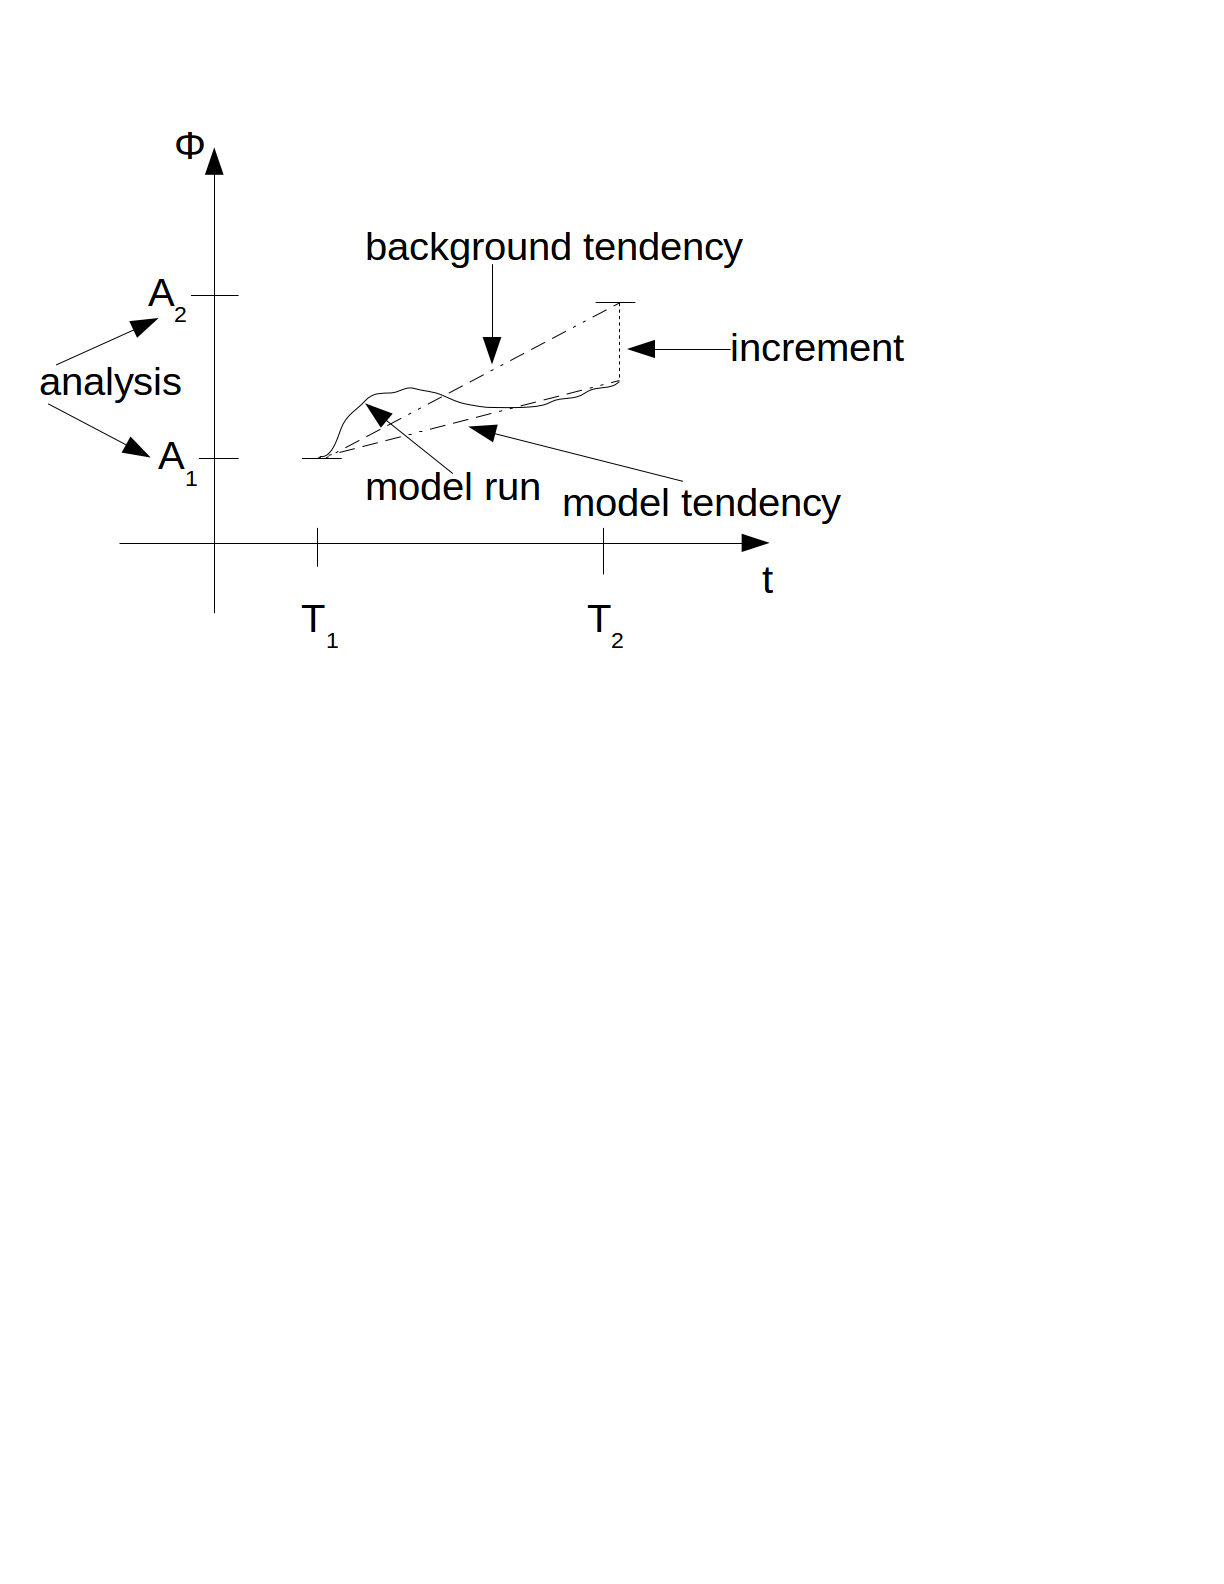
\includegraphics[scale=0.9]{./img/sketch3.png} 

\pagebreak
\section{COSMO Model}
\p
Strict licensing prohibits free use for commercial purposes.

Developed mainly by German weather service (DWD) together with other institutions in the COSMO consortium.

\subsection{Coordinate System}
\subsubsection{Horizontal}
\p
Spherical coordinates with rotated north pole.
\subsubsection{Vertical}
\p
$\cdots$
\subsection{Sound Waves}
\p
Fast time stepping...
\section{WRF Model}
\p
Public domain license.

Developed mainly at NCAR, but everyone is free to participate.
\subsection{Coordinate System}
\subsubsection{Horizontal}
\p
Cartesian, lambert conformal projection
\subsubsection{Vertical}
\p
$\cdots$
\subsection{Sound Waves}
\p
Fast time stepping...
\chapter{Methodology}
\section{Entropy Production}
\subsection{Entropy Temperature}
\begin{equation*}
\text{mixing ratio: }r^t=r^1+r^2+r^3
\end{equation*}
\begin{equation*}
c^*=c_{p0}+c_2r^t
\end{equation*}
\begin{equation*}
a_{21}=R_1T\ln \frac{p^{21}}{p^1}
\end{equation*}
\begin{equation*}
a_{32}=R_1T\ln \frac{p^{31}}{p^{21}}
\end{equation*}
\begin{equation}
\Theta_s=T\qty(\frac{p^0}{p_0})^{-\frac{R_0}{c^*}}\hspace{-0.6cm}\ftimes \exp\qty[\frac{(l_{21}+a_{21})r^1}{c^*T}-\frac{(l_{32}+a_{32})r^3}{c^*T}]
\end{equation}
\subsection{Entropy Production}
\begin{equation}
\dv{s}{t}=m^0c^*\dv{\ln\Theta_s}{t}
\end{equation}
\section{Richardson Number}
\begin{equation*}
\text{Brunt-Väisälä frequency: }N=\sqrt{\frac{g}{\Theta}\dv{\Theta}{z}}
\end{equation*}
\begin{equation}
\Ri=\frac{N^2}{\qty(\dv{u}{z})^2}
\end{equation}
\section{Helicity}
\begin{equation}
H=\int_V \va{v_h}\ftimes\curl{\va{v_h}}
\end{equation}
\section{COSMO}
\subsection{Physics Parameterizations}
Gridscale Precip:\\
4 Graupel scheme with prognostic cloud water, cloud ice, and graupel.

Radiation: Grid- and sub-grid scale (including convective) water and ice clouds are considered; cloud cover, water content and ice content are calculated by the default diagnostic scheme.\\
Coarser grid, every 50 timesteps (=15min)\\
no topographic correction\\
constant aerosol fields, surface albedo is determined by soil type\\

Convection:\\
Shallow convection based on Tiedtke scheme\\
every 10 timesteps (=3min)\\
Convection forcing fields are averaged before calling the scheme.\\
No CAPE or TKE closure\\

Vertical turbulent diffusion:\\
Prognostic TKE-based scheme; includes effects from subgrid-scale condensation/evaporation.\\
Neumann boundary conditions for heat and moisture transport at the lower boundary\\
Grid- and sub-grid scale water clouds are considered\\
No explicit corrections of implicitly calculated turbulent heat and moisture fluxes due to effects from subgrid-scale condensation\\
No consideration of thermal TKE-source in enthalpy budget\\
horizontal turbulent diffusion included\\
calculate SSO-wake turbulence production for TKE\\
don't consider convective buoyancy production for TKE\\
Only vertical shear\\

Surface Layer fluxes:\\
TKE-based scheme including a laminar sub-layer\\
Clouds are not considered for subgridscale condensation\\

Soil Processes:\\
Lake model FLake is not used\\
Terra is run with 7 soil layers\\
2 soil water layers\\
no minimum stomata resistance map\\
BATS is used for transpiration of vegetation and bare soil\\
for heat conductivity an average soil moisture is used.\\

No subgridscale orography is used\\

\section{WRF}
\subsection{Physics Parameterizations}
%\begin{table}
\begin{tabular}{lr}
Microphysics       & New Thompson et al incl. Graupel, rain number density\\
Longwave Radiation & RRTMG (RRTM + random cloud overlap)\\
Shortwave Radiation& RRTMG\\
Clay Surface Layer & Eta similarity (Monin Obukhov)\\
Surface Layer      & Noah land surface model\\
Boundary layer     & Mellor-Yamada-Janjic scheme, 1D TKE + local vert. mixing\\
Cumulus param      & Tiedtke scheme (coarse resolution only)\\
\end{tabular}
%\end{table}
